\documentclass[11pt, a4paper, spanish]{article}

%%%%%%%%%% COMIENZO DEL PREAMBULO %%%%%%%%%%

%Info sobre este documento
\author{Martin Cammi}
\title{Trabajo Pr'actico de Ingenier'ia del software I}

%\usepackage{infostyle}                                                  % provee un look & feel similar a un documento Word
\usepackage[top=2.5cm, bottom=2.5cm, left=2.5cm, right=2.5cm]{geometry}  % m�rgenes
\usepackage[ansinew]{inputenc}                                           % permite que los acentos del estilo ����� salgan joya
\usepackage[spanish, activeacute]{babel}                                 % idioma espa�ol, acentos f�ciles y deletreo de palabras
\usepackage{indentfirst}                                                 % permite indentar un parrafo a mano
\usepackage{caratula}                                                    % incluye caratula est�ndar
\usepackage{graphicx}                                                    % permite insertar gr�ficos
\usepackage{color}                                                       % permite el uso de colores en el documento
\usepackage[pdfcreator={TexLive!, LaTeX2e con TeXnicCenter y la inteligencia de Jonathan ;-)},
			pdfauthor={Grupo 1"},
			pdftitle={Ingenieria del Software - Trabajo practico: sistema de software CentralMarket},
			pdfsubject={Trabajo Practico de Modelado de dominio},
			pdfkeywords={Contenidos, proveedor, bajo demanda},
			pdfstartview=FitH,            % Fits the width of the page to the window
			bookmarksnumbered,            % los bookmarks numerados se ven mejor...
			colorlinks,                   % links con bellos colores
			linkcolor=magenta]            % permite cambiar el color de los links
			{hyperref}                                                         % Permite jugar con algunas cosas que aparecer�n en el PDF final

%\selectlanguage{spanish}

\linespread{1.3}                    % interlineado equivalente al 1.5 l�neas de Word...
\pagestyle{myheadings}              %encabezado personalizable con \markboth{}{}
\markboth{}{Ingenieria del Software - TP de Modelado de Objetivos}
\headsep = 30pt                     % separaci�n entre encabezado y comienzo del p�rrafo

%\addtolength{\oddsidemargin}{-2cm}	% configuracion IDEAL!!!
%\addtolength{\textwidth}{4cm}
%\addtolength{\textheight}{2cm}

% macro 'todo' para To-Do's
\def\todo#1{\textcolor{red}{#1}}

% Macro 'borde' para un texto con borde
\newsavebox{\fmbox}
\newenvironment{borde}[1]
{\begin{lrbox}{\fmbox}\begin{minipage}{#1}}
{\end{minipage}\end{lrbox}\fbox{\usebox{\fmbox}}\\[10pt]}

%%%%%%%%%% FIN DEL PREAMBULO %%%%%%%%%%

\begin{document}

\materia{Ingenier\'ia de Software I}
\submateria{Primer Cuatrimestre de 2012}
\titulo{Trabajo pr\'actico 1}
\subtitulo{An\'alisis preliminar de un sistema de software para CentralMarket}
\grupo{Grupo 1}

\integrante{Abreg\'u, Angel}{082/09}{angelj\_a@hotmail.com}
\integrante{Cammi, Mart\'in}{676/02}{martincammi@gmail.com}
\integrante{De Sousa, Mariano}{389/08}{marian\_sabianaa@hotmail.com}
\integrante{M�ndez, Gonz\'alo}{843/04}{gemm83@hotmail.com}
\integrante{Raffo, Diego}{423/08}{enanodr@hotmail.com}


\maketitle

\thispagestyle{empty}

\tableofcontents

\newpage

% Conviene poner las secciones como diferentes archivos,
% sobre todo cuando se trabaja en equipo.
% Es m�s f�cil para sincronizar mediante control de versiones.
%\input{Introducci�n}


% BEGIN Ejemplos de uso

	%\section{Una secci�n}
	%\label{sec:unaSeccion}
	%Hola! Soy una Secci�n
	%	\subsection{Una subsecci�n}
	%		Y yo soy una subsecci�n!!!
	%		\subsubsection{Una subsubsecci�n}
	%			Y yo soy una sub-subsecci�n!!!
	%			\paragraph{Un p�rrafo\\}
	%				Y yo soy un p�rrafo, porque no hay mas sub-sub-sub-subsecciones!!!

	%\section{Otra secci�n}
	%	Como pudimos ver en la secci�n \ref{sec:unaSeccion}, esto es una demo de una referencia a una secci�n.
	
	%	Tambi�n podemos hacer referencia a la p�gina de la secci�n:\\[10pt]
	
		% Ejemplo de uso de un borde (falta pulir para que no tire un warning!)
	%	\begin{borde}{0.98\textwidth}
	%		En la p�gina \pageref{sec:unaSeccion}, hay una secci�n pilla...
	%	\end{borde}

% END Ejemplos de uso


\section{Propuesta de servicios}
\label{sec:Propuesta de servicios}

\subsection{Introducci\'on}

	La presente propuesta se basa en el documento descripto por el cliente donde describe sus necesitades y requisitos.

	En base a dicho documento hemos identificado una serie de conceptos que para representarlos m�s claramente utilizaremos un \emph{Modelo de Objetivos} que permitir� plasmar claramente las ideas.

	Luego de una elicitaci\'on con el cliente hemos logrado resumir lo que quiere en: \\

	\emph{Mantener un sistema de servicio de contenido digital por internet 
	gratuito y pago bajo demanda para generar ingresos,  personalizado, 
	que sea transparente y tenga calidad de contenido}
	\\
	Los principales Objetivos que vemos son importantes para el cliente son:\\
	transparente
	calidad

\newpage
	
\section{Alcance del sistema}

\subsection{Diagrama de Contexto}

	******Explicar la relaci\'on del sistema con los usuarios hardware y otros sistemas.*****

	A continuaci\'on describimos los principales \emph{agentes} que intervendr\'an en el \emph{Sistema} mediante el Modelo de Jackson.
	En \'el tambi\'en puede observarse la interfaz del \emph{Sistema} y que \emph{agentes} son los que intervienen directamente.

	\begin{center}
		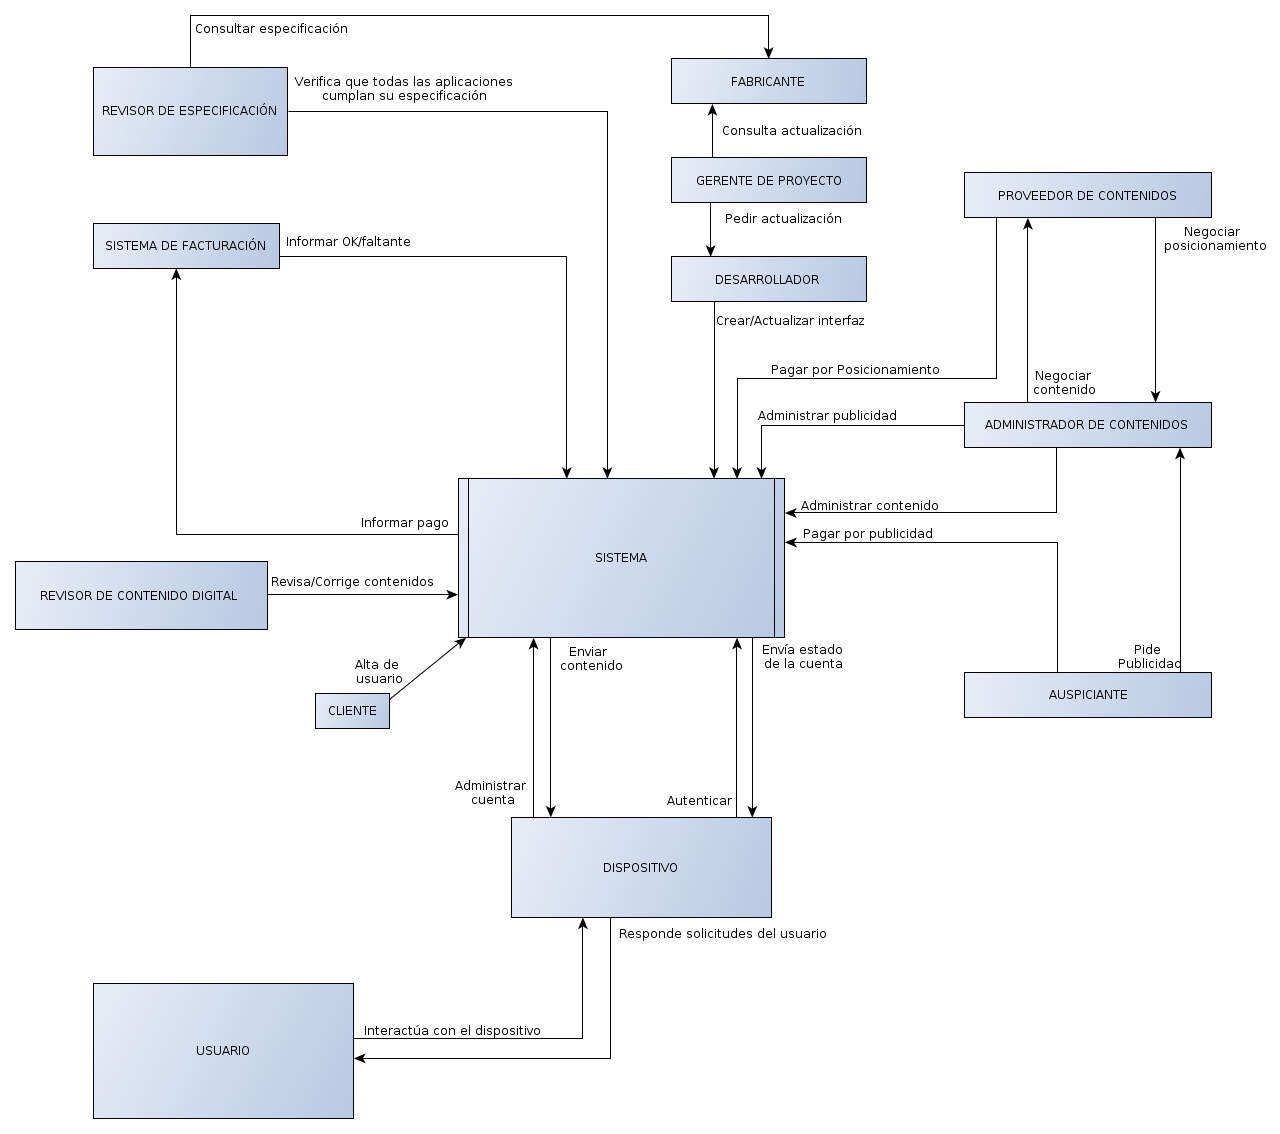
\includegraphics[scale=0.35]{Diagramas/DiagramaContexto.png}
	\end{center}

	El \emph{Sistema} se relaciona con varios agentes tanto directa como indirectamente. Ellos son:

	- Usuario: es la cuenta desde la cual el cliente se conectar\'a al sistema.
	El usuario interact\'ua con el sistema pudiendo autenticarse y Administrar su cuenta.

		El cliente puede mediante la cuenta de usuario autenticarse para ser identificado en el sistema.
		Administrar el contenido engloba las siguientes acciones:

		- Comprar contenido
		- Prestar contenido
    		- Pedir contenido

	- 
	
\section{Objetivos del sistema}

\subsection{Modelo de Objetivos del sistema}

	A continuaci\'on describimos el Modelo de Objetivos que proponemos para cumplir los objetivos detallados anteriormente.
	\begin{center}
		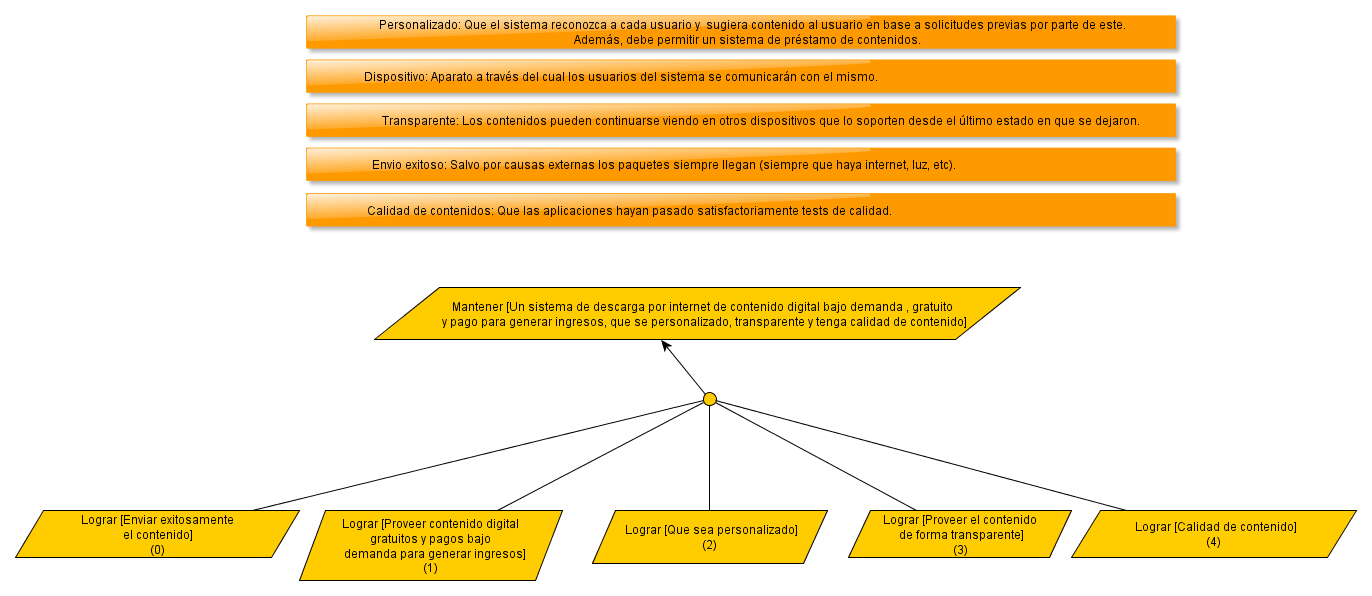
\includegraphics[scale=0.35]{Diagramas/ModelodeObjetivosPrincipal.png}
	\end{center}
	
\subsection{Objetivos blandos}

\section{Asunciones}

	Dentro del sistema una cuenta de usuario no puede reproducir m\'as de un contenido por cuenta.
	Si otro contenido 

\section{Escenarios informales y ejemplos}
	
	Caso1
	Caso2
	Caso3

	Colocar texto de escenarios y ejemplos.



\end{document}
